%% Standard start of a latex document
\documentclass[letterpaper,12pt]{article}
%% Always use 12pt - it is much easier to read
% \usepackage{algorithm}
% \usepackage{algpseudocode}
\usepackage{float}
\usepackage{xcolor}

%% AMS mathematics packages - they contain many useful fonts and symbols.
\usepackage{amsmath, amsfonts, amssymb}
\usepackage{graphicx}
\usepackage[linesnumbered, ruled, vlined]{algorithm2e}
\usepackage{amsmath}

%% The geometry package changes the margins to use more of the page, I suggest
%% using it because standard latex margins are chosen for articles and letters,
%% not homework.
\usepackage[paper=letterpaper,left=25mm,right=25mm,top=3cm,bottom=25mm]{geometry}
%% For details of how this package work, google the ``latex geometry documentation''.

\usepackage{enumerate}
%%
%% Fancy headers and footers - make the document look nice
\usepackage{fancyhdr} %% for details on how this work, search-engine ``fancyhdr documentation''
% \pagestyle{fancy}
%%
%% This is a little more complicated because we have used `` \\ '' to force a line-break between the name and number.
%%
\newcommand{\Z}{\mathbb{Z}}
\newcommand{\bigO}{\mathcal{O}}

\cfoot{Page \thepage} % page in middle

%% These put horizontal lines between the main text and header and footer.
\renewcommand{\footrulewidth}{0.4pt}
%%%

%%%%%%
%% We shouldnt have to change the stuff above, but if you want to add some newcommands and things like that, then putting them between here and the ``\begin{document}'' is a good idea.
%%%%%%


\begin{document}
% Homework 0 does not contain any mathematics --- it is just for you to practice using latex. All I want you to do is to try to reproduce this document as well as you can. You do not have to hand it in. I don't mind if you work in small groups, but just copying it directly from a friend isn't going to help you later in the term.

\begin{center}
    {\LARGE \textbf{Examples}} \\
    First Draft
\end{center}

\

In this file, I will try to run through some examples 
for ratio 1, 2, and 3 with our program so far. 
For outputs of ratio 2, the array represents different $kmax = n+1,\dots$.
For outputs of ratio 3, each line represents different values of $e$
(the bound on $p$-valuation of the determinant of the solution), and for each $e$,
the array represents the ratio for $k = 1, \dots, n$ in order.
The following runtime may be inaccurate as (for some unknown reason),
running Julia in WSL (Windows Subsystem for Linux) can cause inconsistent runtime 
(as much as a factor of 3!).
The examples are as follows,
\begin{enumerate}
\item $p=2, n=7, M' = \begin{pmatrix}
1 & 0 \\ 0 & 3
\end{pmatrix}.$ \\
For $kmax = 8, \dots, 15$, we get \\
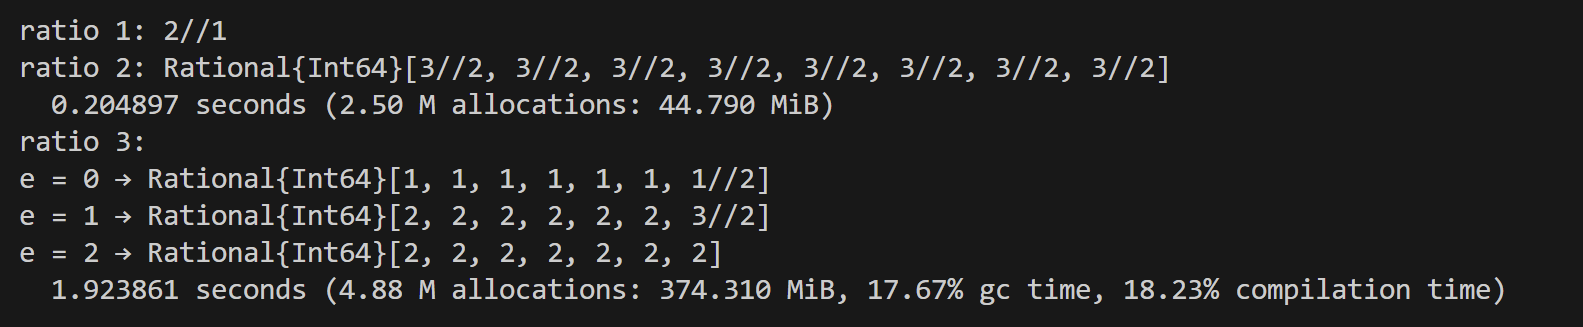
\includegraphics[scale=0.4]{ex1.png} \\

\item $p=2, n=7, M' = \begin{pmatrix}
1 & 0 \\ 0 & 5
\end{pmatrix}.$ \\
For $kmax = 8, \dots, 15$, we get \\
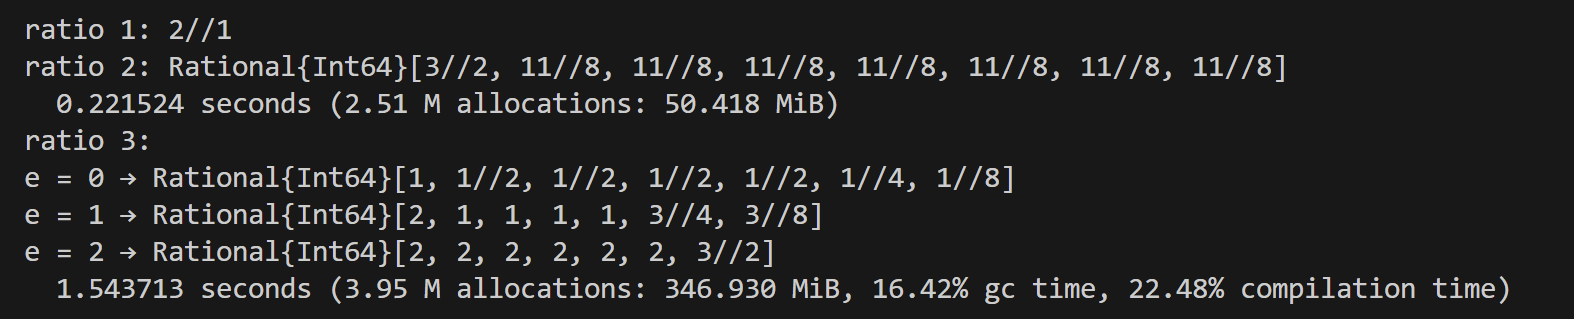
\includegraphics[scale=0.4]{ex2.png} \\

\item $p=2, n=8, M' = \begin{pmatrix}
1 & 0 \\ 0 & 5
\end{pmatrix}.$ \\
For $kmax = 9, \dots, 15$, we get \\
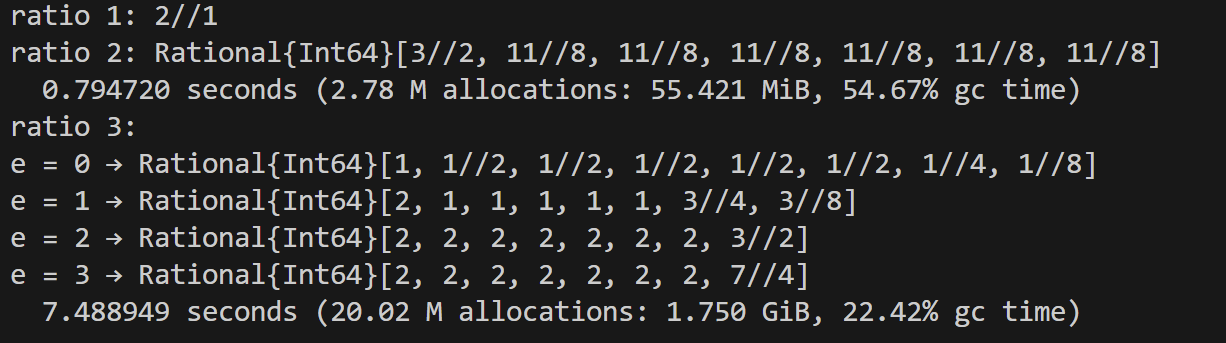
\includegraphics[scale=0.4]{ex3.png} \\

\item $p=2, n=9, M' = \begin{pmatrix}
1 & 0 \\ 0 & 5
\end{pmatrix}.$ \\
For $kmax = 10, \dots, 15$, we get \\
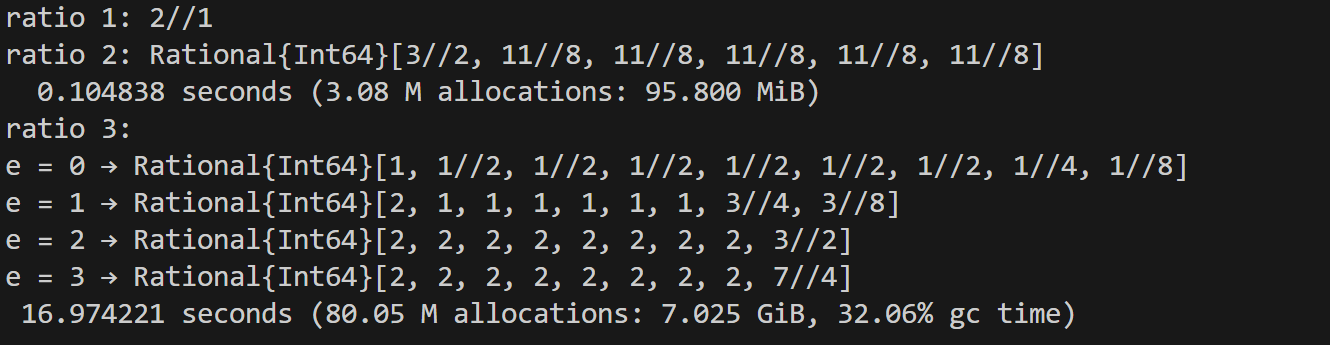
\includegraphics[scale=0.4]{ex4.png} \\

\item $p=2, n=10, M' = \begin{pmatrix}
1 & 0 \\ 0 & 5
\end{pmatrix}.$ \\
For $kmax = 11, \dots, 15$, we get \\
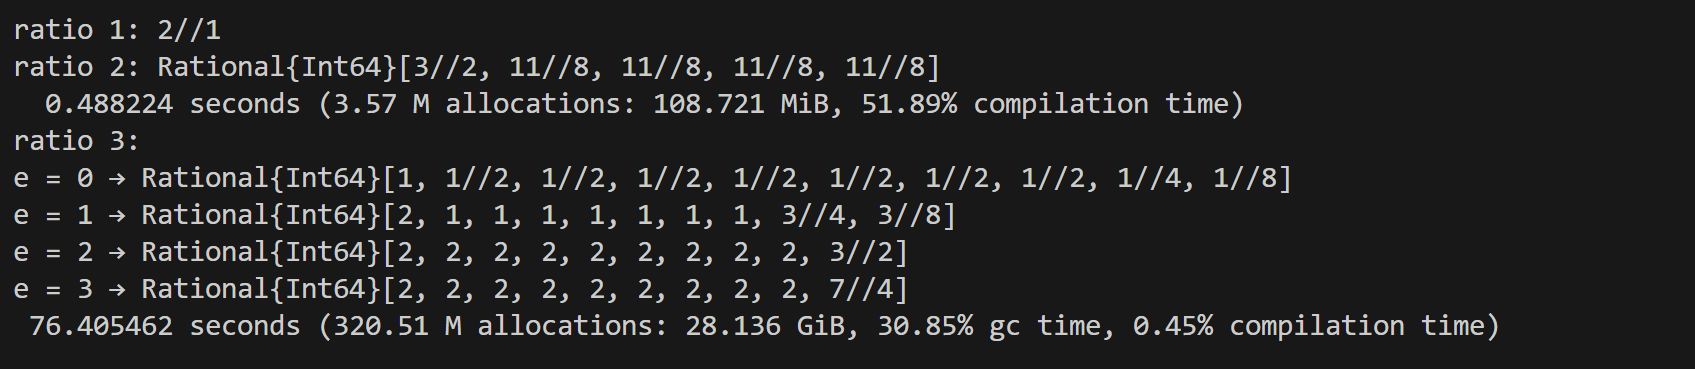
\includegraphics[scale=0.4]{ex5.png} \\

\item $p=2, n=11, M' = \begin{pmatrix}
1 & 0 \\ 0 & 5
\end{pmatrix}.$ \\
For $kmax = 12, \dots, 15$, we get \\
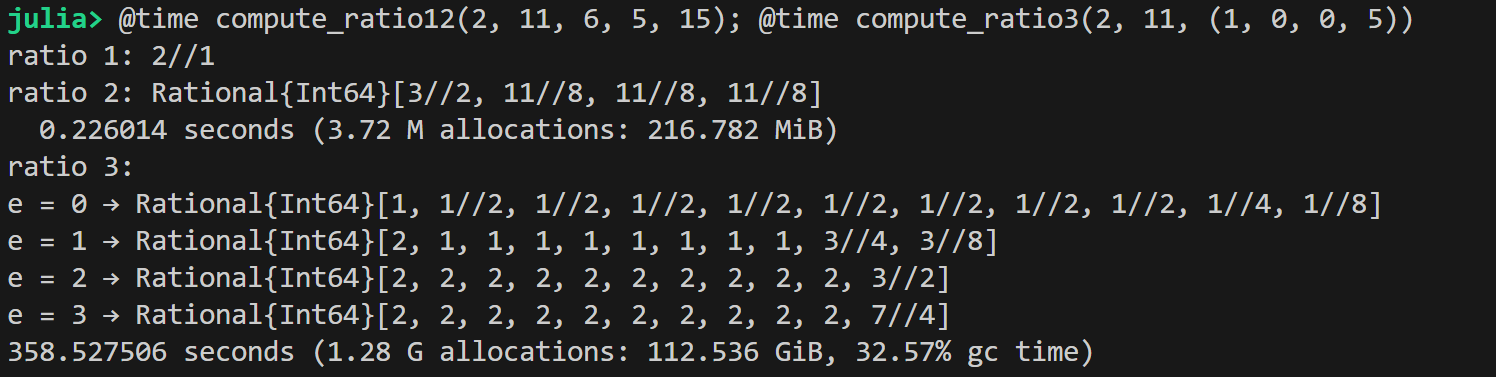
\includegraphics[scale=0.4]{ex8.png} \\

\item $p=2, n=10, M' = \begin{pmatrix}
1 & 0 \\ 0 & 9
\end{pmatrix}.$ \\
For $kmax = 11, \dots, 15$, we get \\
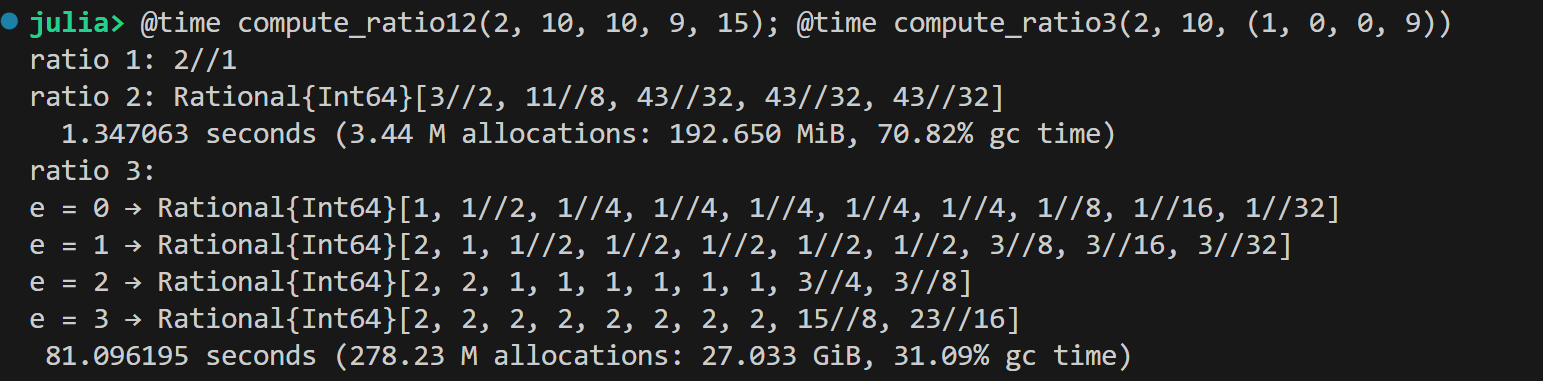
\includegraphics[scale=0.4]{ex6.png} \\

\item $p=2, n=11, M' = \begin{pmatrix}
1 & 0 \\ 0 & 9
\end{pmatrix}.$ \\
For $kmax = 12, \dots, 15$, we get \\
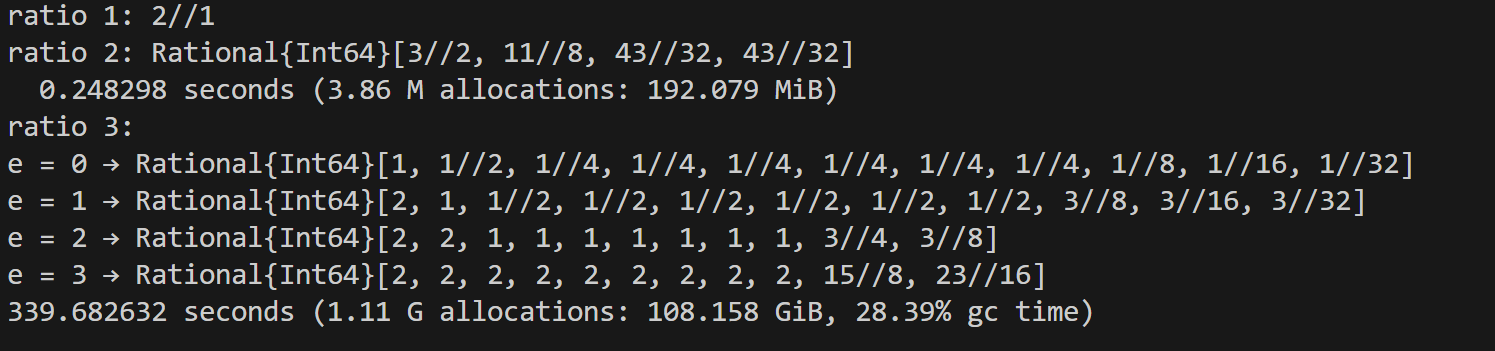
\includegraphics[scale=0.4]{ex7.png} \\

\item $p=3, n=6, M' = \begin{pmatrix}
1 & 0 \\ 0 & 4
\end{pmatrix}.$ \\
For $kmax = 7, \dots, 12$, we get \\
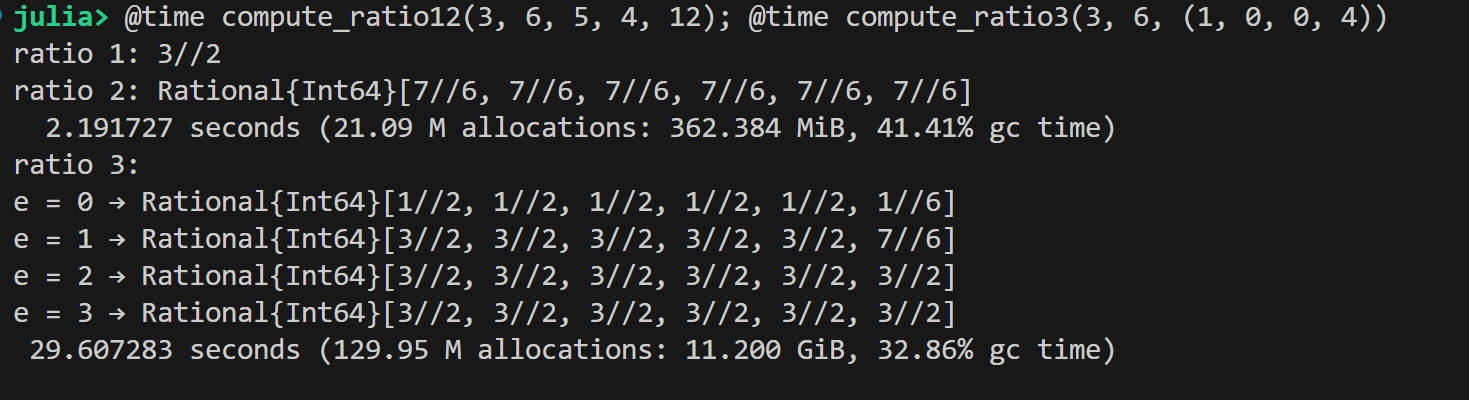
\includegraphics[scale=0.4]{ex9.png} \\

\item $p=3, n=6, M' = \begin{pmatrix}
1 & 0 \\ 0 & 10
\end{pmatrix}.$ \\
For $kmax = 7, \dots, 12$, we get \\
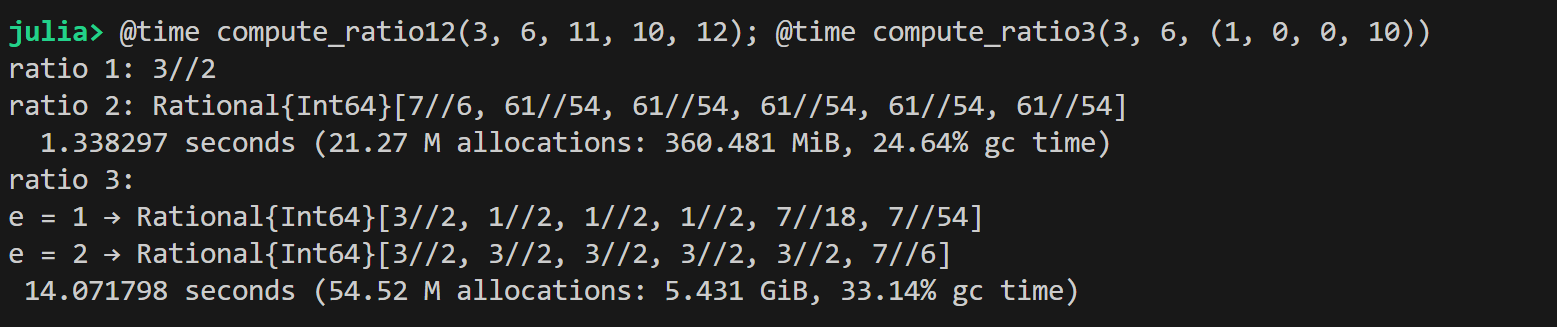
\includegraphics[scale=0.4]{ex10.png} \\

\item $p=3, n=7, M' = \begin{pmatrix}
1 & 0 \\ 0 & 10
\end{pmatrix}.$ \\
For $kmax = 8, \dots, 12$, we get \\
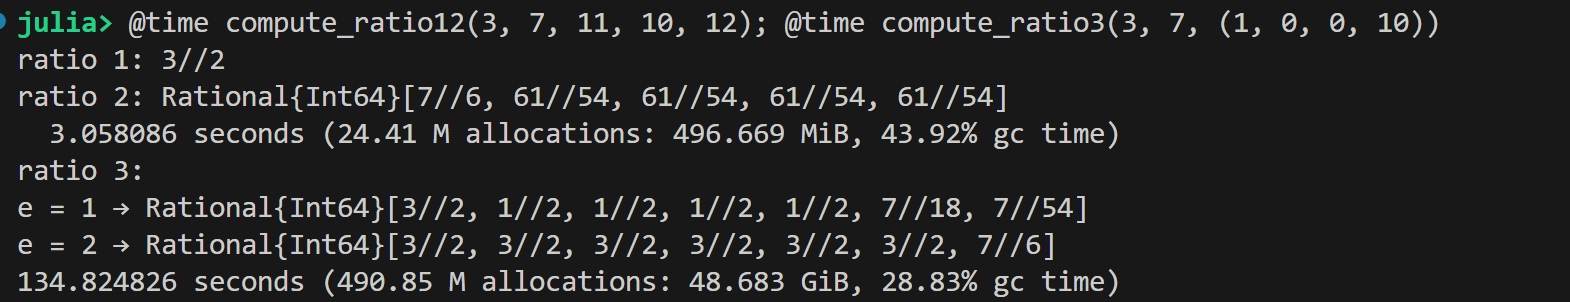
\includegraphics[scale=0.4]{ex11.png} \\

\item $p=3, n=7, M' = \begin{pmatrix}
1 & 0 \\ 0 & 28
\end{pmatrix}.$ \\
For $kmax = 8, \dots, 12$, we get \\
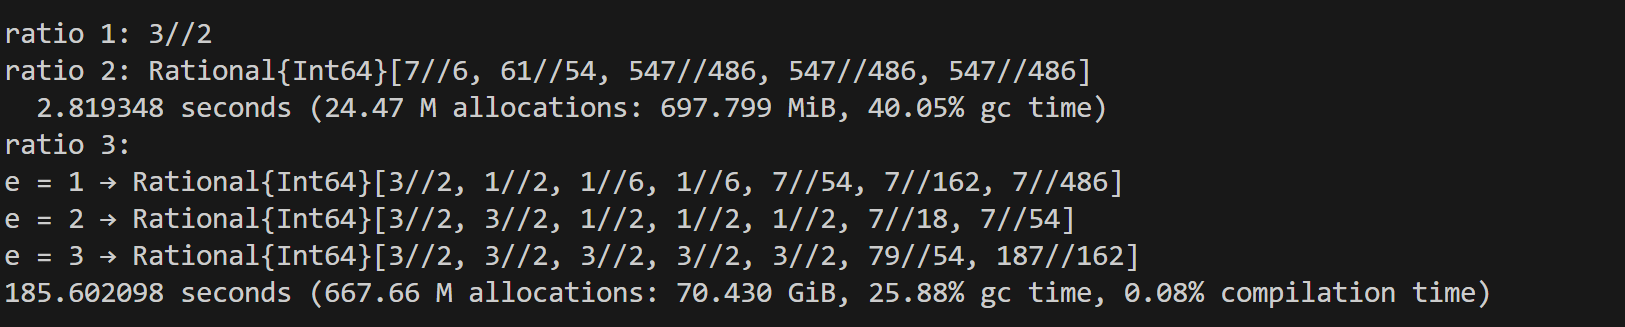
\includegraphics[scale=0.4]{ex12.png} \\

\item $p=3, n=7, M' = \begin{pmatrix}
1 & 6 \\ 3 & 1
\end{pmatrix}.$ \\
For $kmax = 8, \dots, 12$, we get \\
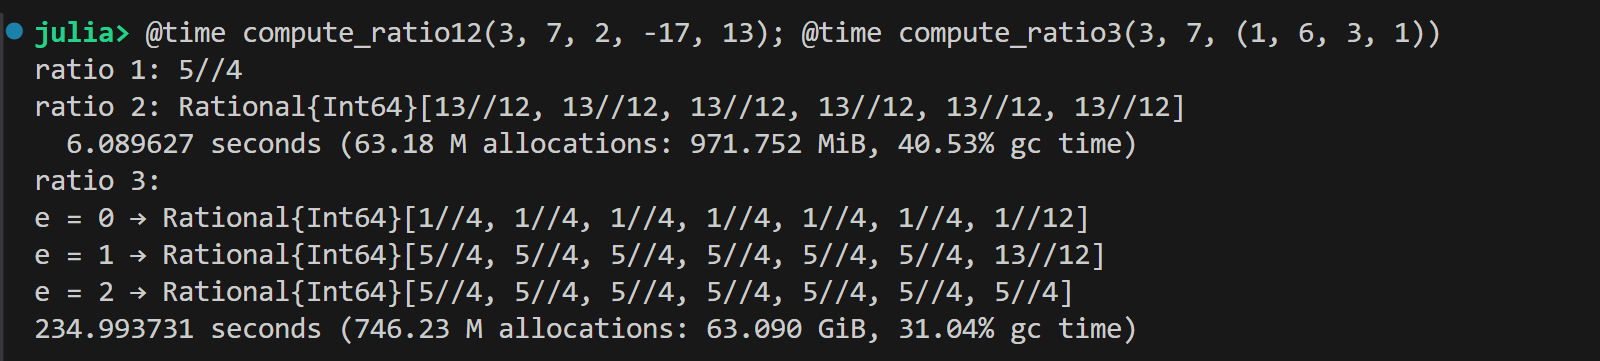
\includegraphics[scale=0.4]{ex13.png} \\

\item $p=3, n=7, M' = \begin{pmatrix}
1 & 18 \\ 9 & 1
\end{pmatrix}.$ \\
For $kmax = 8, \dots, 12$, we get \\
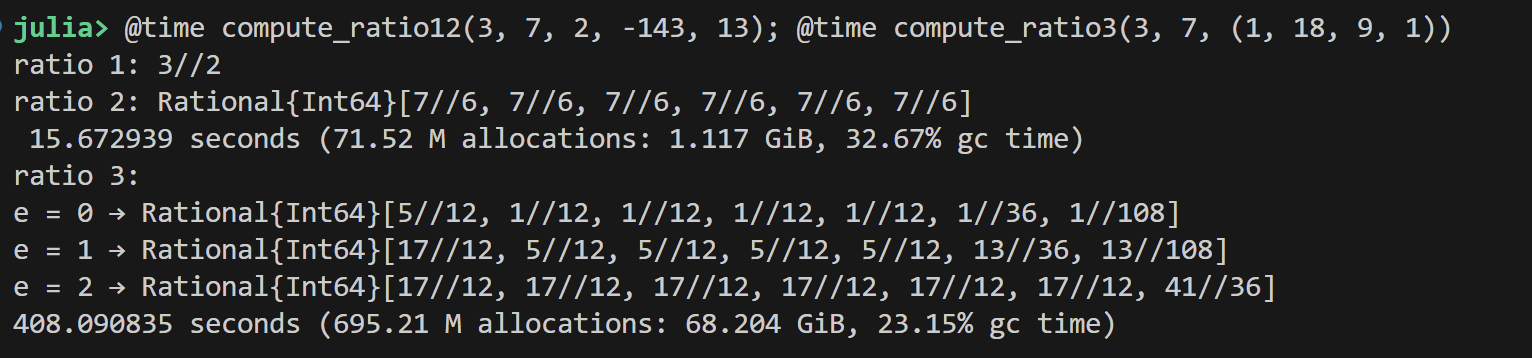
\includegraphics[scale=0.4]{ex14.png} \\

\item $p=5, n=5, M' = \begin{pmatrix}
1 & 0 \\ 0 & 6
\end{pmatrix}.$ \\
For $kmax = 6, \dots, 9$, we get \\
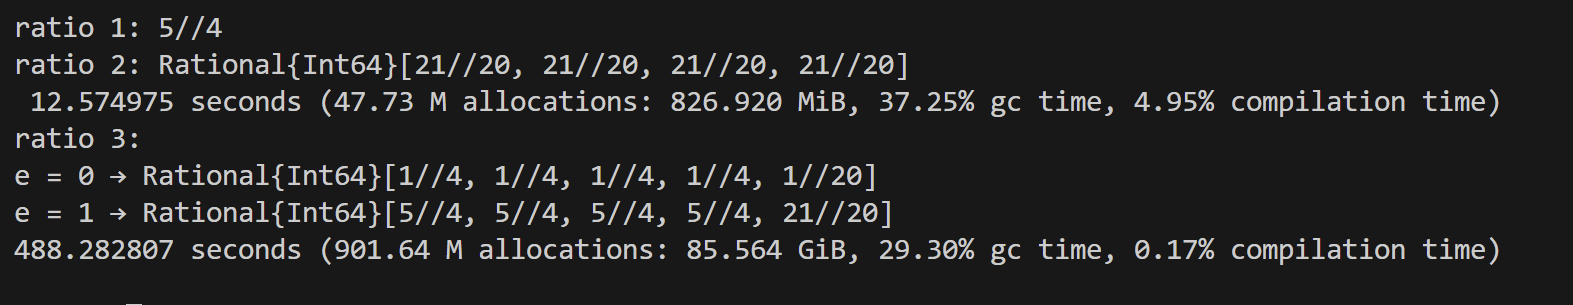
\includegraphics[scale=0.4]{ex15.png} \\

\item $p=5, n=5, M' = \begin{pmatrix}
1 & 10 \\ 5 & 1
\end{pmatrix}.$ \\
For $kmax = 6, \dots, 9$, we get \\
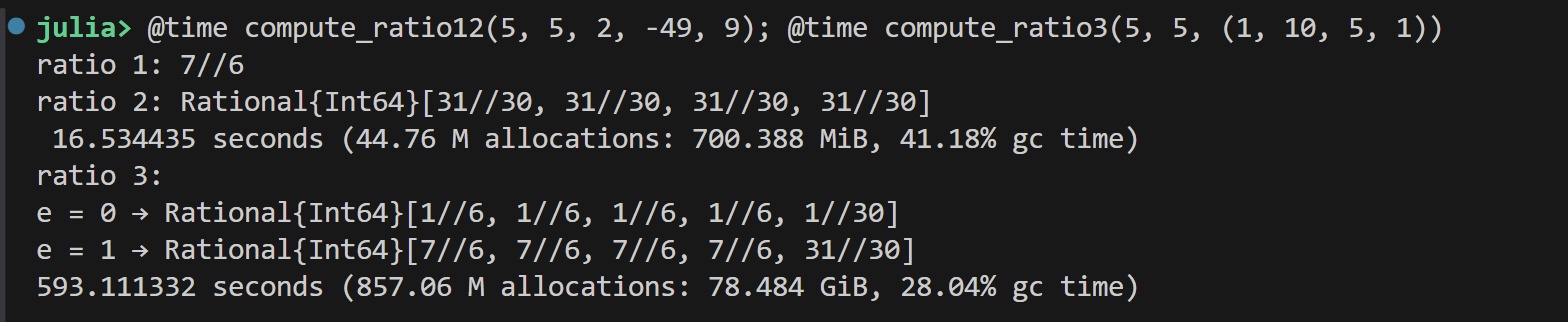
\includegraphics[scale=0.4]{ex16.png} \\

\end{enumerate}

%% Anything that comes after the ``\end{document}'' will be ignored.
\end{document}
